\documentclass[aspectratio=169, xcolor={usenames, dvipsnames}]{beamer}
\usetheme[titleformat=plain, % supported values: plain
          logo=i12en,        % supported values: i12en (default), i12de
          itemsize=20pt,
          % defaultitemsep=0.4\baselineskip,
         ]{itc}

% Encoding and language
\usepackage[utf8]{inputenc}
\usepackage[T1]{fontenc}
\usepackage[english]{babel}
\usepackage{listings, listings-rust}
\usepackage{tikz}
\usetikzlibrary{decorations.pathreplacing}
\usepackage[dvipsnames]{xcolor}

% Meta information
\title{Visualization of Data Movements and Accesses}
\author{Til Mohr}
% Optional, appears on title page
\presenter{Til Mohr}
\institute{IT Center}
\date{September 25\textsuperscript{th} \& 26\textsuperscript{th}, 2023}

\begin{document}

\lstdefinestyle{mycstyle}{
	language=Rust,
	breaklines=true,
	showstringspaces=false,
	keywordstyle=\color{blue},
	commentstyle=\color{green!50!black},
	%escapeinside=||,
	basicstyle=\ttfamily,
	morecomment=[l][{\color{red!50!black}}]{\#},
	backgroundcolor=\color{black!4},
	numbers=left,
	numbersep=10pt,
	numberstyle=\footnotesize,
	framexleftmargin=0.1cm,
	xrightmargin=0.75cm,
	xleftmargin=0.75cm,
	frame=lines,
	tabsize=4,
	belowskip=0cm,
}


\begin{frame}[plain]
\titlepage
\end{frame}

\begin{frame}[fragile]{Sum of Matrix Elements}
\begin{columns}[T] % align columns
\begin{column}{.48\textwidth}
\begin{lstlisting}[style=mycstyle, caption={Matrix Summation}, escapechar=!]
let matrix = Matrix::random(2, 2);
let mut sum = 0;
for !{\color{ForestGreen} column}! in !{\color{ForestGreen} 0..2}! {
  for !{\color{red} row}! in !{\color{red} 0..2}! {
    sum += matrix.get(!{\color{red} row}!, !{\color{ForestGreen} column}!);
  }
}
sum
\end{lstlisting}
\hfill
\end{column}%
\hfill%
\begin{column}{.48\textwidth}
\begin{tikzpicture}[
	box/.style={rectangle,draw=black,thick, minimum size=1cm},
]
	\draw[step=1cm,color=gray] (0,0) grid (2,2);
	\node[box,fill=CornflowerBlue] at (0.5,0.5) {3};
	\node[box,fill=CornflowerBlue] at (1.5,0.5) {4};
	\node[box,fill=Goldenrod] at (0.5,1.5) {1};
	\node[box,fill=Goldenrod] at (1.5,1.5) {2};
	\node at (-0.5,1.5) {\color{red} 0};
	\node at (-0.5,0.5) {\color{red} 1};
	\node at (0.5,2.5) {\color{ForestGreen} 0};
	\node at (1.5,2.5) {\color{ForestGreen} 1};
	\node[below right] at (-0.5,4) {Matrix:};

	\only<2->{
		\draw[step=1cm,color=gray] (5,1) grid (4+5,2);
		\node[box,fill=Goldenrod] at (5.5,1.5) {1};
		\node[box,fill=Goldenrod] at (6.5,1.5) {2};
		\node[box,fill=CornflowerBlue] at (7.5,1.5) {3};
		\node[box,fill=CornflowerBlue] at (8.5,1.5) {4};
		\draw[color=gray,line width=3pt] (5,1) rectangle (2+5,2);
		\draw[color=gray,line width=3pt] (2+5,1) rectangle (4+5,2);
		\node[below right] at (-0.5+5,4) {Matrix in Memory:};

		\only<3-4>{
			% Element (0,0)
			\draw[color=black,line width=4pt] (0,1) rectangle (1,2);
			\draw[color=black,line width=4pt] (5,1) rectangle (6,2);
		}
		\only<5-6>{
			% Element (1,0)
			\draw[color=black,line width=4pt] (0,0) rectangle (1,1);
			\draw[color=black,line width=4pt] (7,1) rectangle (8,2);
		}
		\only<7-8>{
			% Element (0,1)
			\draw[color=black,line width=4pt] (1,1) rectangle (2,2);
			\draw[color=black,line width=4pt] (6,1) rectangle (7,2);
		}
		\only<9-10>{
			% Element (1,1)
			\draw[color=black,line width=4pt] (1,0) rectangle (2,1);
			\draw[color=black,line width=4pt] (8,1) rectangle (9,2);
		}
	}

	\only<3->{
		\draw[step=1cm,color=gray] (0,2-5) grid (2,3-5);
		\node[below right] at (-0.5,4.25-5) {Current Item:};
		\only<3-4>{
			\node at (0.5,2.5-5) {\color{red} 0};
			\node at (1.5,2.5-5) {\color{ForestGreen} 0};
		}
		\only<5-6>{
			\node at (0.5,2.5-5) {\color{red} 1};
			\node at (1.5,2.5-5) {\color{ForestGreen} 0};
		}
		\only<7-8>{
			\node at (0.5,2.5-5) {\color{red} 0};
			\node at (1.5,2.5-5) {\color{ForestGreen} 1};
		}
		\only<9-10>{
			\node at (0.5,2.5-5) {\color{red} 1};
			\node at (1.5,2.5-5) {\color{ForestGreen} 1};
		}

		\draw[step=1cm,color=gray] (0+5,2-5) grid (2+5,3-5);
		\node[below right] at (-0.5+5,4.25-5) {Cache:};

		\only<4-5>{
			% Line [(0,0), (0,1)] in cache
			\node[box,fill=Goldenrod] at (0.5+5,2.5-5) {1};
			\node[box,fill=Goldenrod] at (1.5+5,2.5-5) {2};

			\only<4>{
				\draw[decorate,decoration={brace,amplitude=8pt,mirror,raise=4ex}] (5,2) -- (7,2) node[midway] {};
				\draw[->,line width=1pt] (6,0.4) to [out=270,in=30] (7,-2);
				\draw[color=black,line width=4pt] (0+5,2-5) rectangle (1+5,3-5);
			}
		}

		\only<6-7>{
			% Line [(1,0), (1,1)] in cache
			\node[box,fill=CornflowerBlue] at (0.5+5,2.5-5) {3};
			\node[box,fill=CornflowerBlue] at (1.5+5,2.5-5) {4};

			\only<6>{
				\draw[decorate,decoration={brace,amplitude=8pt,mirror,raise=4ex}] (7,2) -- (9,2) node[midway] {};
				\draw[->,line width=1pt] (8,0.4) to [out=270,in=30] (7,-2);
				\draw[color=black,line width=4pt] (0+5,2-5) rectangle (1+5,3-5);
			}
		}

		\only<8-9>{
			% Line [(0,1), (0,2)] in cache
			\node[box,fill=Goldenrod] at (0.5+5,2.5-5) {1};
			\node[box,fill=Goldenrod] at (1.5+5,2.5-5) {2};

			\only<8>{
				\draw[decorate,decoration={brace,amplitude=8pt,mirror,raise=4ex}] (5,2) -- (7,2) node[midway] {};
				\draw[->,line width=1pt] (6,0.4) to [out=270,in=30] (7,-2);
				\draw[color=black,line width=4pt] (1+5,2-5) rectangle (2+5,3-5);
			}
		}

		\only<10>{
			% Line [(1,1), (1,2)] in cache
			\node[box,fill=CornflowerBlue] at (0.5+5,2.5-5) {3};
			\node[box,fill=CornflowerBlue] at (1.5+5,2.5-5) {4};

			\only<10>{
				\draw[decorate,decoration={brace,amplitude=8pt,mirror,raise=4ex}] (7,2) -- (9,2) node[midway] {};
				\draw[->,line width=1pt] (8,0.4) to [out=270,in=30] (7,-2);
				\draw[color=black,line width=4pt] (1+5,2-5) rectangle (2+5,3-5);
			}
		}
	}
\end{tikzpicture}

\end{column}%
\end{columns}
\vfill
\only<3>{
	\begin{center}
		Number of cache misses: \textbf{0}
	\end{center}
}
\only<4-5>{
	\begin{center}
		Number of cache misses: \textbf{1}
	\end{center}
}
\only<6-7>{
	\begin{center}
		Number of cache misses: \textbf{2}
	\end{center}
}
\only<8-9>{
	\begin{center}
		Number of cache misses: \textbf{3}
	\end{center}
}
\only<10>{
	\begin{center}
		Number of cache misses: \textbf{4}
	\end{center}
}
\end{frame}

\begin{frame}[fragile]{Sum of Matrix Elements - Reordered Loops}
\begin{columns}[T] % align columns
\begin{column}{.48\textwidth}
\begin{lstlisting}[style=mycstyle, caption={Matrix Summation}, escapechar=!]
let matrix = Matrix::random(2, 2);
let mut sum = 0;
for !{\color{red} row}! in !{\color{red} 0..2}! {
  for !{\color{ForestGreen} column}! in !{\color{ForestGreen} 0..2}! {
	sum += matrix.get(!{\color{red} row}!, !{\color{ForestGreen} column}!);
  }
}
sum
\end{lstlisting}
\hfill
\end{column}%
\hfill%
\begin{column}{.48\textwidth}
\begin{tikzpicture}[
	box/.style={rectangle,draw=black,thick, minimum size=1cm},
]
	\draw[step=1cm,color=gray] (0,0) grid (2,2);
	\node[box,fill=CornflowerBlue] at (0.5,0.5) {3};
	\node[box,fill=CornflowerBlue] at (1.5,0.5) {4};
	\node[box,fill=Goldenrod] at (0.5,1.5) {1};
	\node[box,fill=Goldenrod] at (1.5,1.5) {2};
	\node at (-0.5,1.5) {\color{red} 0};
	\node at (-0.5,0.5) {\color{red} 1};
	\node at (0.5,2.5) {\color{ForestGreen} 0};
	\node at (1.5,2.5) {\color{ForestGreen} 1};
	\node[below right] at (-0.5,4) {Matrix:};

	\only<1->{
		\draw[step=1cm,color=gray] (5,1) grid (4+5,2);
		\node[box,fill=Goldenrod] at (5.5,1.5) {1};
		\node[box,fill=Goldenrod] at (6.5,1.5) {2};
		\node[box,fill=CornflowerBlue] at (7.5,1.5) {3};
		\node[box,fill=CornflowerBlue] at (8.5,1.5) {4};
		\draw[color=gray,line width=3pt] (5,1) rectangle (2+5,2);
		\draw[color=gray,line width=3pt] (2+5,1) rectangle (4+5,2);
		\node[below right] at (-0.5+5,4) {Matrix in Memory:};

		\only<1-2>{
			% Element (0,0)
			\draw[color=black,line width=4pt] (0,1) rectangle (1,2);
			\draw[color=black,line width=4pt] (5,1) rectangle (6,2);
		}
		\only<3>{
			% Element (0,1)
			\draw[color=black,line width=4pt] (1,1) rectangle (2,2);
			\draw[color=black,line width=4pt] (6,1) rectangle (7,2);
		}
		\only<4-5>{
			% Element (1,0)
			\draw[color=black,line width=4pt] (0,0) rectangle (1,1);
			\draw[color=black,line width=4pt] (7,1) rectangle (8,2);
		}
		\only<6>{
			% Element (1,1)
			\draw[color=black,line width=4pt] (1,0) rectangle (2,1);
			\draw[color=black,line width=4pt] (8,1) rectangle (9,2);
		}
	}

	\only<1->{
		\draw[step=1cm,color=gray] (0,2-5) grid (2,3-5);
		\node[below right] at (-0.5,4.25-5) {Current Item:};
		\only<1-2>{
			\node at (0.5,2.5-5) {\color{red} 0};
			\node at (1.5,2.5-5) {\color{ForestGreen} 0};
		}
		\only<3>{
			\node at (0.5,2.5-5) {\color{red} 0};
			\node at (1.5,2.5-5) {\color{ForestGreen} 1};
		}
		\only<4-5>{
			\node at (0.5,2.5-5) {\color{red} 1};
			\node at (1.5,2.5-5) {\color{ForestGreen} 0};
		}
		\only<6>{
			\node at (0.5,2.5-5) {\color{red} 1};
			\node at (1.5,2.5-5) {\color{ForestGreen} 1};
		}

		\draw[step=1cm,color=gray] (0+5,2-5) grid (2+5,3-5);
		\node[below right] at (-0.5+5,4.25-5) {Cache:};

		\only<2-3>{
			% Line [(0,0), (0,1)] in cache
			\node[box,fill=Goldenrod] at (0.5+5,2.5-5) {1};
			\node[box,fill=Goldenrod] at (1.5+5,2.5-5) {2};

			\only<2>{
				\draw[decorate,decoration={brace,amplitude=8pt,mirror,raise=4ex}] (5,2) -- (7,2) node[midway] {};
				\draw[->,line width=1pt] (6,0.4) to [out=270,in=30] (7,-2);
				\draw[color=black,line width=4pt] (0+5,2-5) rectangle (1+5,3-5);
			}

			\only<3>{
				\draw[color=black,line width=4pt] (1+5,2-5) rectangle (2+5,3-5);
			}

		}

		\only<5-6>{
			% Line [(1,0), (1,1)] in cache
			\node[box,fill=CornflowerBlue] at (0.5+5,2.5-5) {3};
			\node[box,fill=CornflowerBlue] at (1.5+5,2.5-5) {4};

			\only<5>{
				\draw[decorate,decoration={brace,amplitude=8pt,mirror,raise=4ex}] (7,2) -- (9,2) node[midway] {};
				\draw[->,line width=1pt] (8,0.4) to [out=270,in=30] (7,-2);
				\draw[color=black,line width=4pt] (0+5,2-5) rectangle (1+5,3-5);
			}

			\only<6>{
				\draw[color=black,line width=4pt] (1+5,2-5) rectangle (2+5,3-5);
			}
		}
	}
\end{tikzpicture}

\end{column}%
\end{columns}
\vfill
\only<1>{
	\begin{center}
		Number of cache misses: \textbf{0}
	\end{center}
}
\only<2-4>{
	\begin{center}
		Number of cache misses: \textbf{1}
	\end{center}
}
\only<5-6>{
	\begin{center}
		Number of cache misses: \textbf{2}
	\end{center}
}
\end{frame}

\begin{frame}{Outline}
\tableofcontents
\end{frame}

\section{Memory-Related Performance Problems}
\subsection{Data Locality}
\subsection{Processor-Memory Performance Gap}

\section{Overview of the Optimization Workflow}

\section{Data Gathering Approaches}

\section{Visualization Techniques}

\section{Specific Optimization Tool}

\section{Conclusion}



\end{document}
